\documentclass{handout}

\SetInstructor{Lt Col James Phillips}
\SetCourseTitle{ECE231: Electrical Circuits and Systems I}
\SetSemester{Block II}
\SetHandoutTitle{Lecture 15: Operational Amplifiers - Part 2
}
%\SetDueDate{1 Jan 2016}
%\ShowAllBlanks

\showsoln \setsolncolor{red}

\begin{document}
\maketitle

\textbf{OBJECTIVES:}
\begin{enumerate}
\item Starting with the ideal Op Amp model, develop circuits for Summing and Subtracting Amplifiers
\end{enumerate}

\textbf{READING}
\begin{description}
\item [Required]:
\begin{itemize}
\item  Textbook, section 4.4, pages 190--201
\end{itemize}
\item [Optional]: None
\end{description}

\section{The Summing Amplifier}
Often in circuit design, we will need to add to signals together -- this CANNOT be down by simply connecting two wires, although many of you in your solutions will try that method.  To add two signals we must use a device called an {\em adder} or {\em summing amplifier}.   In this section we will design a weighted (and inverting) summing amplifier.

\subsection{Derivation}
Let's start by looking at the inverting Op Amp discussed in last class (see Figure \ref{fig: InvertingOpAmp})

\begin{figure} [h! t! b!]
\centering
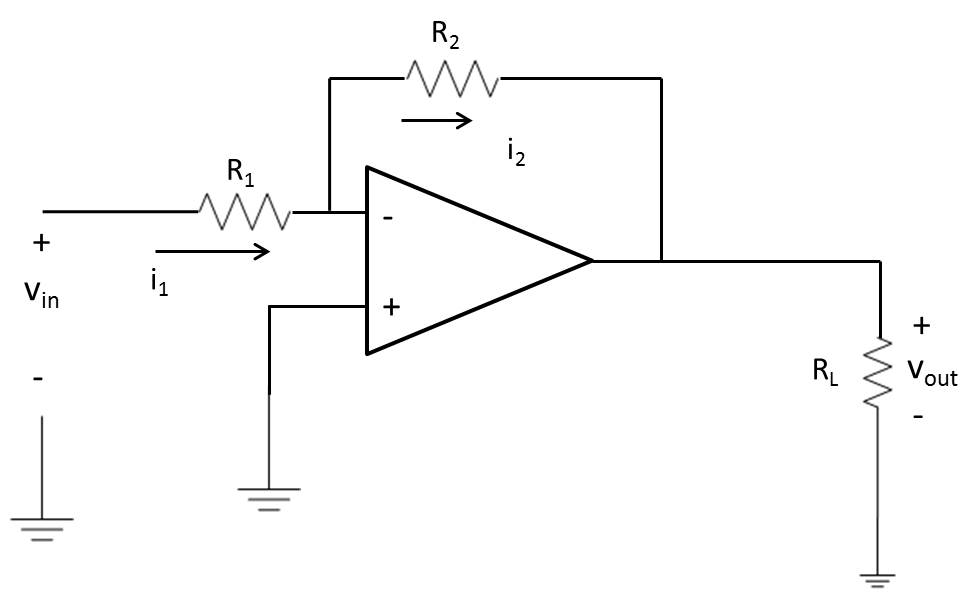
\includegraphics[width=0.5\textwidth]{InvertingOpAmp.jpg}
\caption{Inverting Op Amp}
\label{fig: InvertingOpAmp}
\end{figure}

Recall that the transfer characterisitic for this amplifier is:
\begin{equation}
\frac{V_{out}}{V_{in}}=-\frac{R_2}{R_1}
\end{equation}
which can also be written as
\begin{equation}
V_{out}=-\frac{V_{in}}{R_1}R_2
\end{equation}
but since $\frac{V_{in}}{R_1} = i_1$ we can say the output voltage is really determined by the input current, $i_1$.

\textbf{Are there other ways of increasing the input current without increaseing $V_{in}$?}
Consider the circuit shown in Figure \ref{fig: InvertingSummer}
\begin{figure} [h!]
\centering
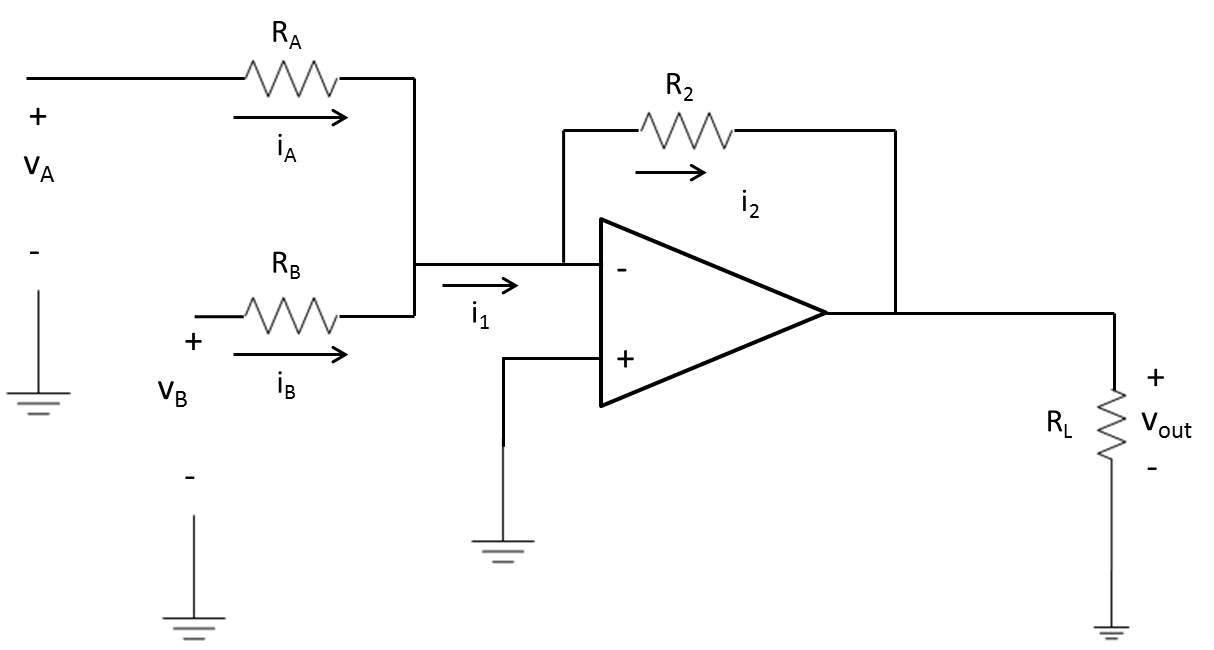
\includegraphics[width=0.7\textwidth]{InvertingSummer.jpg}
\caption{Inverting Summer}
\label{fig: InvertingSummer}
\end{figure}

The output voltage is still fully determined by the input current, $i_1$; but now $i_1$ is the {\em sum} of two currents, $i_A$ and $i_B$.

Let's derive a transfer characteristic of this amplifier circuit that relates $V_{out}$ to $V_A$ and $V_B$.

\soln{6in}{
Start by writing a KCL equation at the inverting terminal
\begin{equation}
i_A + i_B = i_2 + i_n
\end{equation}
but we know $i_n=0$ so
\begin{equation}
i_A + i_B = i_2
\end{equation}
Since we also know that $v_n=0$ we can write $i_A$ and $i_B$ interms of $V_A$ and $V_B$
\begin{equation}
\frac{V_A}{R_A} + \frac{V_B}{R_B} = i_2
\end{equation}
We recall from last lesson that
\begin{equation}
V_{out}=-i_2R_2
\end{equation}
whic combining the last 2 equations gives
\begin{equation}
\frac{V_A}{R_A} + \frac{V_B}{R_B} = \frac{-V_{out}}{R_2}
\end{equation}
which solving for $V_{out}$ gives
\begin{equation}
V_{out}=-\left(\frac{R_2}{R_A}V_A + \frac{R_2}{R_B}V_B \right)
\end{equation}
Thus the name {\em weighted, inverting summer}
}

This derivation is easily extended to an arbritrary number of inputs.

A block diagram of a summer is shown in Figure \ref{fig: SummerBlockDiagram}.  It should be noted that the gains ($K_1$ and $K_2$) are typically negative in our implementation

\begin{figure} [h!]
\centering
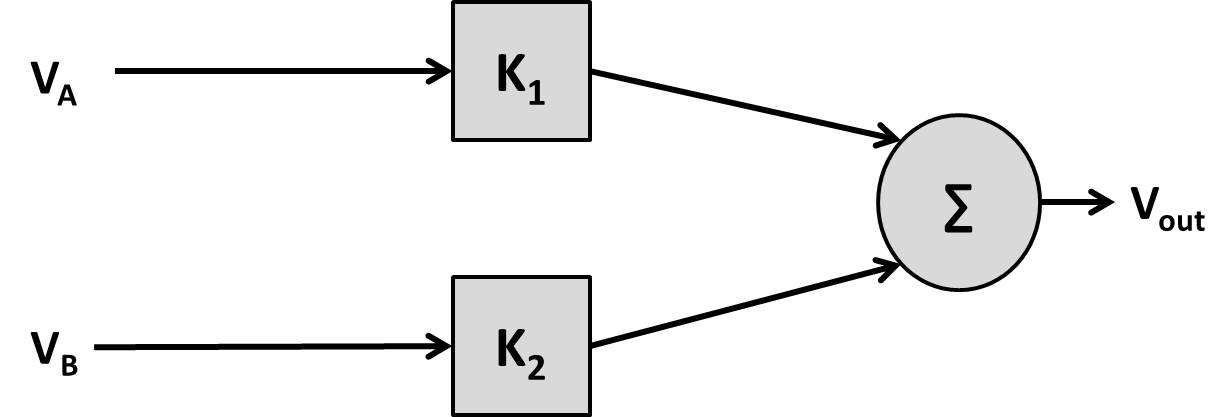
\includegraphics[width=0.7\textwidth]{SummerBlockDiagram.jpg}
\caption{Summer Block Diagram}
\label{fig: SummerBlockDiagram}
\end{figure}

\subsection{Examples}

\textbf{Textbook Design Example 4-16}
Design an inverting summer (refer to Figure \ref{fig: InvertingSummer}) that implements the following transfer characteristic:
\begin{equation}
V_{out} = -(5V_A + 13 V_B)
\end{equation}

\soln{3in}{
Looking back at the transfer characteristic for an inverting summer we know we need the resistances to satisfy the following relationships
\begin{equation}
\frac{R_2}{R_A} = 5
\end{equation}
\begin{equation}
\frac{R_2}{R_B} = 13
\end{equation}
If we limit ourself to standard resistance values, we can start by selecting a value for $R_2$.  Lets let $R_2 = 91\ k\Omega$.  We can then solve for $R_A$ and $R_B$ and select the closest standard value.  It is always good to verify that you are within about 5\% of your desired gain.  We select $R_A = 18\ k\Omega$ and $R_B=6.8\ k\Omega$.  These values yield gains of
\begin{equation}
K_1=\frac{91\ k\Omega}{18\ k\Omega} = 5.0556
\end{equation}
\begin{equation}
K_2 = \frac{91\ k\Omega}{6.8\ k\Omega} = 13.3824
\end{equation}
}

\textbf{Textbook Exercise 4-23}

(a) For the design above find $V_{out}$ if $V_A=2\ V$ and $V_B = -0.5\ V$

(b) If $V_A=500\ mV$ and $V_{CC} = 15\ V$, what is the maximum value of $V_B$ for linear operation?

\soln{3in}{
part (a) is just plug and chug
\begin{equation}
V_{out} = -\left(K_1V_A + K_2V_B \right)= -\left(5.05 \times 2\ V + 13.38 \times (-0.5) \right)= -3.41\ V
\end{equation}

for part (b) we know $|V_{out}| \le 15\ V$.  If we set $V_{out}=15\ V$ in the transfer characteristic equation and solve for $V_B$ we get:
\begin{equation}
V_B = -\frac{V_{out}+K_1V_A}{K_2} = -\frac{15\ V+5.05 \times 500\ mV}{13.38}=-1.31\ V
\end{equation}
If we set $V_{out}=-15\ V$ in the transfer characteristic equation and solve for $V_B$ we get:
\begin{equation}
V_B = -\frac{V_{out}+K_1V_A}{K_2} = -\frac{-15\ V+5.05 \times 500\ mV}{13.38}=932\ mV
\end{equation}
After checking both edges, pick the largest.  Intuition may have allowed you to select the largest without doing both calculations.
}

\newpage
\clearpage
\pagebreak

\section{The Differential Amplifier or Subtractor}
To understand the differential amplifier, let's start with the block diagram shown in Figure \ref{fig: DifferentialAmplifier}.  Notice this block diagram is very similar to the summer block diagram, except that one of the inputs in into an {\em inverting terminal}.

\begin{figure} [h!]
\centering
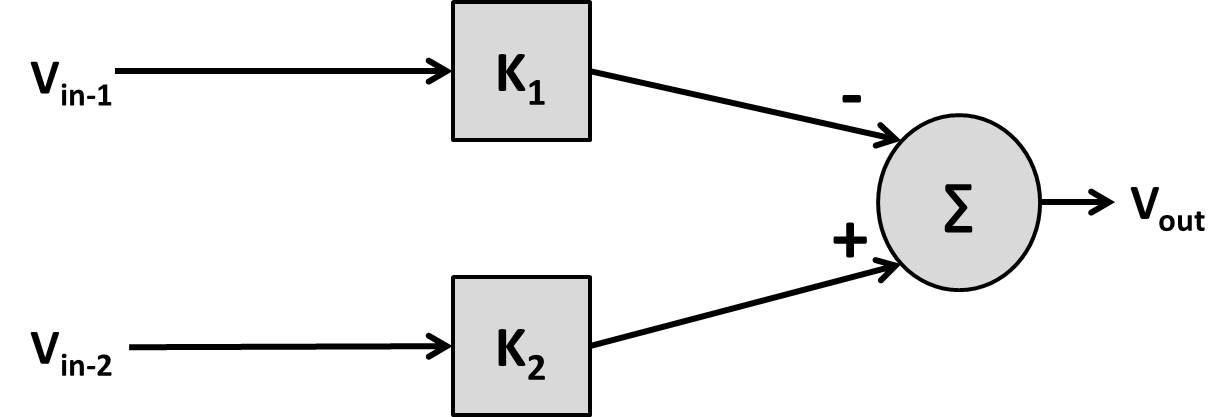
\includegraphics[width=0.7\textwidth]{DifferentialAmplifier.jpg}
\caption{Differential Amplifier Block Diagram}
\label{fig: DifferentialAmplifier}
\end{figure}

\subsection{Derivation}
Rather than try to design a differential amplifier, I will give you the circuit (see Figure \ref{fig: DifferentialAmplifierCircuit}) and then we can derive the transfer characteristic.

\begin{figure} [h!]
\centering
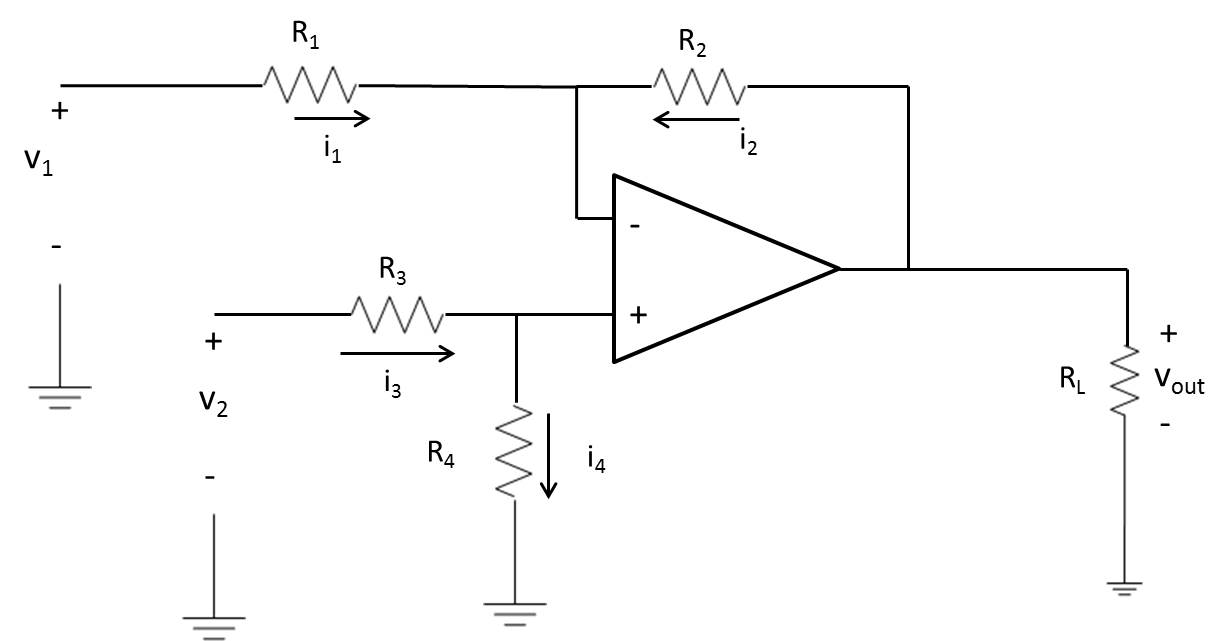
\includegraphics[width=0.7\textwidth]{DifferentialAmplifierCircuit.jpg}
\caption{Differential Amplifier  Circuit Diagram}
\label{fig: DifferentialAmplifierCircuit}
\end{figure}

The derivation below will take advantage of the {\em Superposition} principle.

\newpage
\clearpage
\pagebreak

We will start by {\em turning off} $V_2$ (remember to turn off a voltage source you short it) and finding the output resulting from $V_1$.

\soln{6in}{
With $V_2$ turned off the circuit becomes:
\begin{figure} [h!]
\centering
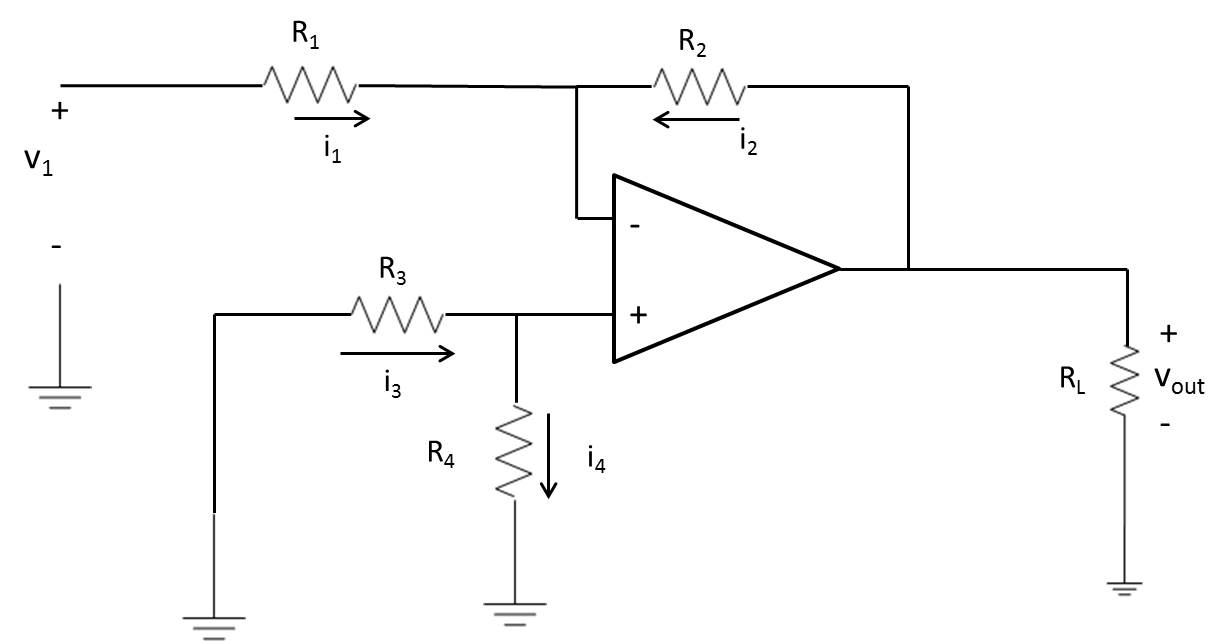
\includegraphics[width=0.7\textwidth]{DifferentialAmplifierCircuitV2off.jpg}
\end{figure}

With $V_2$ off $i_3$ and $i_4$ are zero and the circuit becomes
\begin{figure} [h!]
\centering
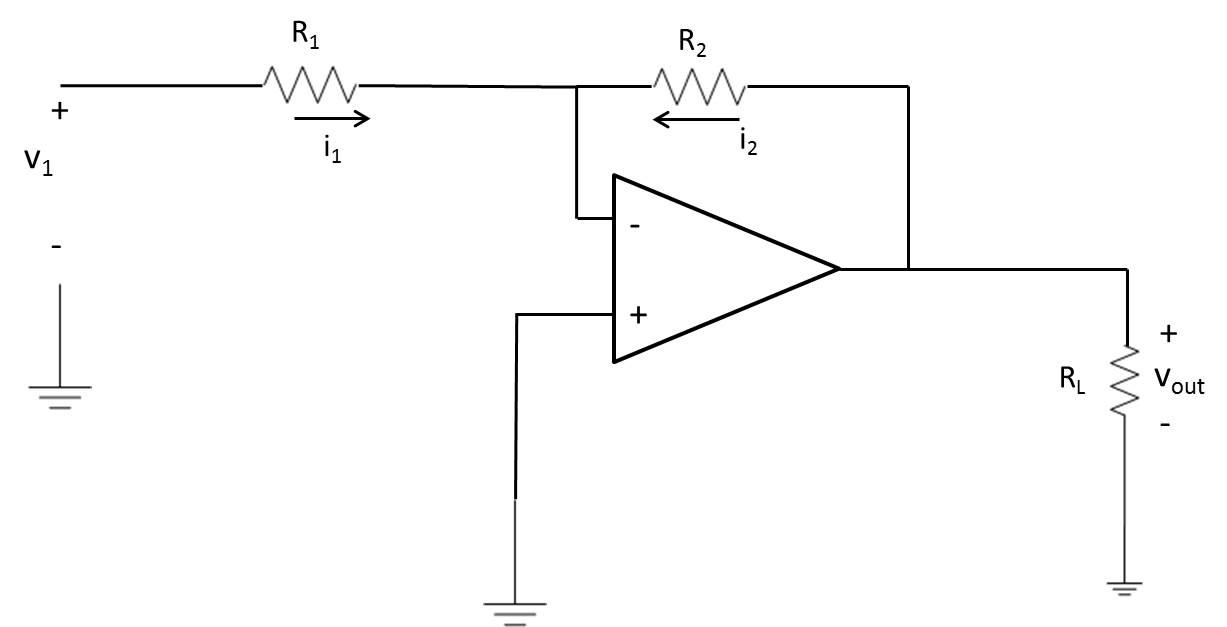
\includegraphics[width=0.7\textwidth]{DifferentialAmplifierCircuitV2off_2.jpg}
\end{figure}
which is easily recognized as an inverting amplifier.  The transfer characteristic is
\begin{equation}
V_{out-1} = -\frac{R_2}{R_1}V_1
\end{equation}
}

\newpage
\clearpage
\pagebreak

Continuing the derivation we now {\em turn off} $V_1$.  The cicuit would now look like

\soln{6in}{

\begin{figure} [h!]
\centering
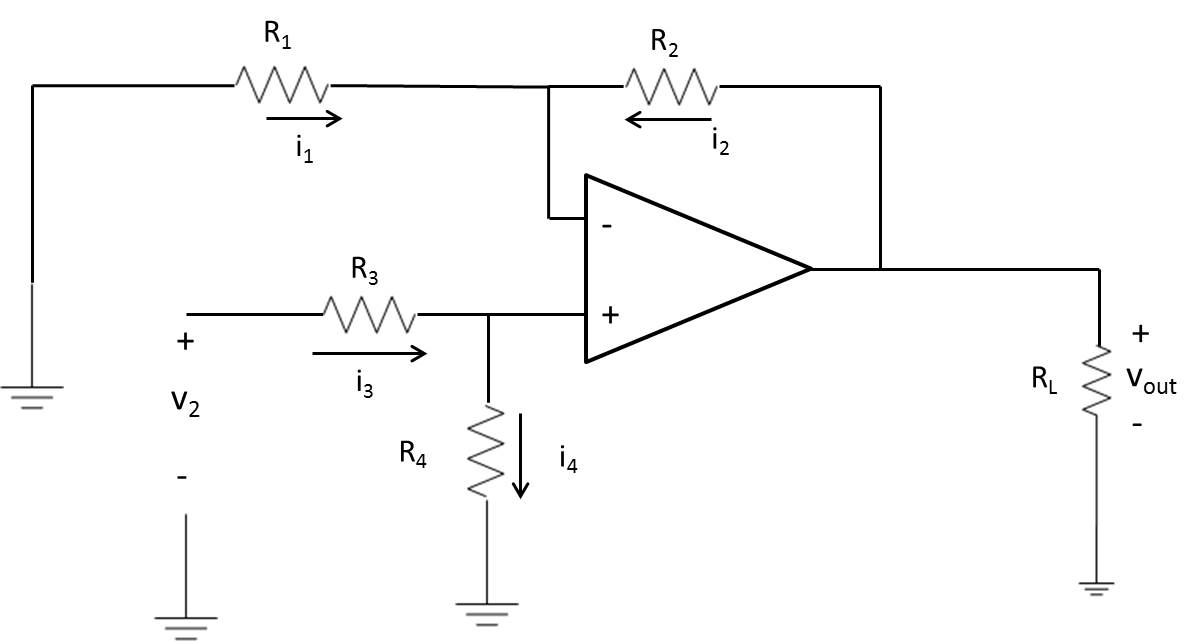
\includegraphics[width=0.7\textwidth]{DifferentialAmplifierCircuitV1off.jpg}
\end{figure}

We now can find the voltage at the non-inverting terminal, $v_p$ using voltage division
\begin{equation}
v_p = \frac{R_4}{R_3+R_4}V_2
\end{equation}
and we know that $v_p = v_n$ therefore
\begin{equation}
v_n = \frac{R_4}{R_3+R_4}V_2
\end{equation}
From here we can solve for $i_1$
\begin{equation}
i_1=-V_2\frac{R_4}{(R_3+R_4)R_1}
\end{equation}
and since $i_1=-i_2$
\begin{equation}
i_2=V_2\frac{R_4}{(R_3+R_4)R_1}
\end{equation}
which means
\begin{equation}
V_{out-2}=V_2\left\{\frac{R_4}{R_3+R_4}V_2 + \frac{R_4R_2}{(R_3+R_4)R_1}\right\} = V_2\left[\frac{R_4}{R_3+R_4}\right]\left[\frac{R_1+R_2}{R_1}\right]
\end{equation}

}

Now that we have the output from $V_1$ and $V_2$ we can add them

\soln{3in}{
\begin{equation}
V_{out} = V_{out-1}+V_{out-2}
\end{equation}
\begin{equation}
V_{out} = -\frac{R_2}{R_1}V_1+\left[\frac{R_4}{R_3+R_4}\right]\left[\frac{R_1+R_2}{R_1}\right]V_2
\end{equation}
so referring back to the block diagram,
\begin{equation}
K_1=\frac{R_2}{R_1}
\end{equation}
Note: We dropped the negatives sign because it is accounted for in the block diagram at the summing junction
\begin{equation}
K_2=\left[\frac{R_4}{R_3+R_4}\right]\left[\frac{R_1+R_2}{R_1}\right]
\end{equation}
}

\newpage
\clearpage
\pagebreak

\subsection{Examples}
\textbf{Textbook Exercise 4-25}

(a) Find the transfer characteristic of a differential amplifier if: $R_1=10\ k\Omega$, $R_2=40\ k\Omega$, $R_3=10\ k\Omega$, and $R_4=15\ k\Omega$.

(b) If $V_{CC} = \pm 15\ V$ and $V_1= 3\ V$ what is the allowable range of $V_2$ for linear operation?

\soln{6in}{
part (a) is plug and chug.... The transfer characteristic written in terms of gains, $K_1$ and $K_2$ is :
\begin{equation}
V_{out} = -K_1V_1+K_2V_2
\end{equation}
solve for gains, $K_1$ and $K_2$
\begin{equation}
K_1=\frac{40\ k\Omega}{10\ k\Omega} = 4
\end{equation}
\begin{equation}
K_2=\left[\frac{15\ k\Omega}{10\ k\Omega+15\ k\Omega}\right]\left[\frac{10\ k\Omega+40\ k\Omega}{10\ k\Omega}\right]=3
\end{equation}
Plugging these gains into the transfer characteristic gives
\begin{equation}
V_{out} = -4V_1+3V_2
\end{equation}

For part (b) we start by solving the transder characteristic for $V_2$
\begin{equation}
V_2 = \frac{V_{out} +4V_1}{3}
\end{equation}
we now solve for the two cases: (1) $V_{out} = 15\ V$, (2) $V_{out} = -15\ V$
\begin{equation}
V_2 = \frac{-15 +(4 \times 3\ V)}{3}= -1\ V
\end{equation}
\begin{equation}
V_2 = \frac{15 +(4 \times 3\ V)}{3}= 9\ V
\end{equation}
therefore
\begin{equation}
-1\ V \le V_2 \le 9\ V
\end{equation}
}





\newpage
\clearpage
\pagebreak

\newpage
\clearpage
\pagebreak

\newpage
\clearpage
\pagebreak

\newpage
\clearpage
\pagebreak

\newpage
\clearpage
\pagebreak

\newpage
\clearpage
\pagebreak

\newpage
\clearpage
\pagebreak

\end{document}


% Equation Array Example Code
%\begin
%{eqnarray}
%P_R &=& i_R^2R \nonumber \\
%P_R &=& (100\ mA)^2 \times 100\ \Omega \nonumber \\
%P_R &=& (100 \times 10^{-3}\ A)^2 \times 100\ \Omega \\
%P_R &=& 10000 \times 10^{-6}\ A^2  \times 100\ \Omega \nonumber \\
%P_R &=& 1\ W  \nonumber
%\end{eqnarray}

% Figure Example Code
%\begin{figure} [h! t! b!]
%\centering
%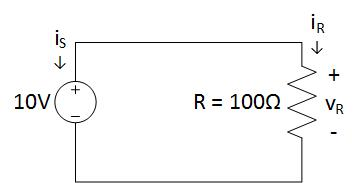
\includegraphics[width=0.5\textwidth]{OhmsLawExampleSolution.jpg}
%\caption{Ohm's Law example circuit}
%\label{fig: OhmsLawExampleSolution}
%\end{figure}

%Table Example Code
%\begin{table}[h]
%\centering
%\begin{tabular}{|l|c|c|}
%\hline
%Prefix & Abbreviation & Value \\
%\hline \hline
%Giga & $G$ & $10^9$ \\
%Mega & $M$ & $10^6$ \\
%Kilo & $k$ & $10^3$ \\
%\hline
%milli & $m$ & $10^{-3}$ \\
%micro & $\mu$ & $10^{-6}$ \\
%nano & $n$ & $10^{-9}$ \\
%pico & $p$ & $10^{-12}$ \\
%\hline
%\end{tabular}
%\caption{Engineering prefixes and values}
%\label{tab: Eng Prefixes}
%\end{table}
